\documentclass{report}
\usepackage[utf8]{inputenc}
\usepackage{graphicx}
\usepackage{here}
%%%\usepackage{color}
\usepackage{rotfloat}

\usepackage{picins}

\usepackage{sidecap}
\usepackage{subfig}

\usepackage{caption}
\captionsetup[figure]{format=hang,labelformat=parens,font={footnotesize,it,color=magenta},margin=3cm}
\captionsetup[table]{indention=4cm,labelsep=endash,labelfont={small,bf,color=red},textfont={small,color=blue},width=8cm,skip=1cm}

\usepackage{diagbox}
\usepackage{multirow}
\usepackage{array}
\setlength{\extrarowheight}{2pt}

\usepackage[x11names,table]{xcolor}
\definecolor{yo}{cmy}{0.6,0.3,0.8}
\usepackage{hhline}

\usepackage{longtable}

\usepackage{bm}

\usepackage{eucal}
\usepackage{mathrsfs}
\usepackage{dsfont}

\usepackage{empheq}

\usepackage{mathtools}

\begin{document}
	
\begin{align}
a+b+c&=\alpha \\
\Aboxed{b+d&=\gamma}
\end{align}
	
	
	
$$
\begin{pmatrix*}[r]
aaaaa & bb & d \\
a & b & ddddddd 
\end{pmatrix*}
$$
	

$$
\underbracket[1.6pt][5mm]{4+4+4+4}_{16}
$$
	
$$
A\xleftrightarrow[c]{a+b}D\xLeftrightarrow[p]{q+r}D
$$	
	
$$
\sum_{\mathclap{i=564563456456}}^{n_0} a_i
$$
	

\begin{empheq}[left=\Rightarrow,right=\Longleftarrow,outerbox=\colorbox{cyan!30}]{align}
a+b+c&=\alpha \\
b+d&=\gamma
\end{empheq}
	
\begin{empheq}[left=\Rightarrow,right=\Longleftarrow,innerbox=\colorbox{yellow}]{align}
a+b+c&=\alpha \\
b+d&=\gamma
\end{empheq}
	
\begin{empheq}[box=\fcolorbox{red}{Orchid1}]{align}
a+b+c&=\alpha \\
b+d&=\gamma
\end{empheq}	
	
	
	
	
$$
\mathds{ABCDEFGHIJKLMNOPQRSTUVWXYZ}
$$	
	
$$
\mathscr{ABCDEFGHIJKLMNOPQRSTUVWXYZ}
$$	
	
$$
\mathcal{ABCDEFGHIJKLMNOPQRSTUVWXYZ}
$$
	
$$
\alpha \bm{\alpha}
$$
	
	
	
\newpage	
	
\begin{longtable}[c]{c|c|c|c}
	\caption{Una tabla muy grande}\\
	\hline
	casa** & mesa** & silla** & libro**\\
	\endfirsthead
	casa* & mesa* & silla* & libro* \\
	\hline
	\endhead
	\multicolumn{4}{r}{continúa...}
	\endfoot	
	\multicolumn{4}{r}{fin}
	\endlastfoot
	casa & mesa & silla & libro \\
	Casa & Mesa & Silla & Libro \\
	CASA & MESA & SILLA & LIBRO \\
	casa & mesa & silla & libro \\
	\pagebreak
	Casa & Mesa & Silla & Libro \\
	CASA & MESA & SILLA & LIBRO \\
	casa & mesa & silla & libro \\
	Casa & Mesa & Silla & Libro \\
	CASA & MESA & SILLA & LIBRO \\
	casa & mesa & silla & libro \\
	Casa & Mesa & Silla & Libro \\
	CASA & MESA & SILLA & LIBRO \\
	casa & mesa & silla & libro \\
	Casa & Mesa & Silla & Libro \\
	CASA & MESA & SILLA & LIBRO \\
	casa & mesa & silla & libro \\
	Casa & Mesa & Silla & Libro \\
	CASA & MESA & SILLA & LIBRO \\
	casa & mesa & silla & libro \\
	Casa & Mesa & Silla & Libro \\
	CASA & MESA & SILLA & LIBRO \\
	casa & mesa & silla & libro \\
	Casa & Mesa & Silla & Libro \\
	CASA & MESA & SILLA & LIBRO \\
	casa & mesa & silla & libro \\
	Casa & Mesa & Silla & Libro \\
	CASA & MESA & SILLA & LIBRO \\
	casa & mesa & silla & libro \\
	Casa & Mesa & Silla & Libro \\
	CASA & MESA & SILLA & LIBRO \\
	casa & mesa & silla & libro \\
	Casa & Mesa & Silla & Libro \\
	CASA & MESA & SILLA & LIBRO \\	
	casa & mesa & silla & libro \\
	Casa & Mesa & Silla & Libro \\
	CASA & MESA & SILLA & LIBRO \\
	casa & mesa & silla & libro \\
	Casa & Mesa & Silla & Libro \\
	CASA & MESA & SILLA & LIBRO \\
	casa & mesa & silla & libro \\
	Casa & Mesa & Silla & Libro \\
	CASA & MESA & SILLA & LIBRO \\
	casa & mesa & silla & libro \\
	Casa & Mesa & Silla & Libro \\
	CASA & MESA & SILLA & LIBRO \\
	casa & mesa & silla & libro \\
	Casa & Mesa & Silla & Libro \\
	CASA & MESA & SILLA & LIBRO \\
	casa & mesa & silla & libro \\
	Casa & Mesa & Silla & Libro \\
	CASA & MESA & SILLA & LIBRO \\
	casa & mesa & silla & libro \\
	Casa & Mesa & Silla & Libro \\
	CASA & MESA & SILLA & LIBRO \\
	casa & mesa & silla & libro \\
	Casa & Mesa & Silla & Libro \\
	CASA & MESA & SILLA & LIBRO \\
	casa & mesa & silla & libro \\
	Casa & Mesa & Silla & Libro \\
	CASA & MESA & SILLA & LIBRO \\
	casa & mesa & silla & libro \\
	Casa & Mesa & Silla & Libro \\
	CASA & MESA & SILLA & LIBRO \\
	casa & mesa & silla & libro \\
	Casa & Mesa & Silla & Libro \\
	CASA & MESA & SILLA & LIBRO \\
	casa & mesa & silla & libro \\
	Casa & Mesa & Silla & Libro \\
	CASA & MESA & SILLA & LIBRO \\
	casa & mesa & silla & libro \\
	Casa & Mesa & Silla & Libro \\
	CASA & MESA & SILLA & LIBRO \\
	casa & mesa & silla & libro \\
	Casa & Mesa & Silla & Libro \\
	CASA & MESA & SILLA & LIBRO \\
	casa & mesa & silla & libro \\
	Casa & Mesa & Silla & Libro \\
	CASA & MESA & SILLA & LIBRO \\
	casa & mesa & silla & libro \\
	Casa & Mesa & Silla & Libro \\
	CASA & MESA & SILLA & LIBRO \\
	casa & mesa & silla & libro \\
	Casa & Mesa & Silla & Libro \\
	CASA & MESA & SILLA & LIBRO \\
	casa & mesa & silla & libro \\
	Casa & Mesa & Silla & Libro \\
	CASA & MESA & SILLA & LIBRO \\
	casa & mesa & silla & libro \\
	Casa & Mesa & Silla & Libro \\
	CASA & MESA & SILLA & LIBRO \\
	casa & mesa & silla & libro \\
	Casa & Mesa & Silla & Libro \\
	CASA & MESA & SILLA & LIBRO \\
	casa & mesa & silla & libro \\
	Casa & Mesa & Silla & Libro \\
	CASA & MESA & SILLA & LIBRO \\
	casa & mesa & silla & libro \\
	Casa & Mesa & Silla & Libro \\
	CASA & MESA & SILLA & LIBRO \\
	casa & mesa & silla & libro \\
	Casa & Mesa & Silla & Libro \\
	CASA & MESA & SILLA & LIBRO \\
	casa & mesa & silla & libro \\
	Casa & Mesa & Silla & Libro \\
	CASA & MESA & SILLA & LIBRO \\
	casa & mesa & silla & libro \\
	Casa & Mesa & Silla & Libro \\
	CASA & MESA & SILLA & LIBRO \\
	casa & mesa & silla & libro \\
	Casa & Mesa & Silla & Libro \\
	CASA & MESA & SILLA & LIBRO \\
	casa & mesa & silla & libro \\
	Casa & Mesa & Silla & Libro \\
	CASA & MESA & SILLA & LIBRO \\
	casa & mesa & silla & libro \\
	Casa & Mesa & Silla & Libro \\
	CASA & MESA & SILLA & LIBRO \\
	casa & mesa & silla & libro \\
	Casa & Mesa & Silla & Libro \\
	CASA & MESA & SILLA & LIBRO \\
	casa & mesa & silla & libro \\
	Casa & Mesa & Silla & Libro \\
	CASA & MESA & SILLA & LIBRO \\
	\hline
\end{longtable}	
	
	
	
	
	
	
\newpage	
	
\begin{tabular}{|c|c|c|c|}
	\hline
\rowcolor{green} & mesa & silla & libro \\
\hhline{|>{\arrayrulecolor{green}}->{\arrayrulecolor{black}}|---}
\rowcolor{green} 	\multirow{-2}{*}{HOY}	 & Mesa & Silla & Libro \\
	CASA & MESA & SILLA & LIBRO \\
	\hline
\end{tabular}

\ \\[2cm]
	
\begin{table}[H]
\rowcolors{3}{yellow!30}{cyan!30}
\begin{tabular}{c|c|c|c}
	\hline
	casa & mesa & silla & libro \\
	Casa & Mesa & Silla & Libro \\
	CASA & MESA & SILLA & LIBRO \\
	casa & mesa & silla & libro \\
	Casa & Mesa & Silla & Libro \\
	CASA & MESA & SILLA & LIBRO \\
	casa & mesa & silla & libro \\
	Casa & Mesa & Silla & Libro \\
	CASA & MESA & SILLA & LIBRO \\
	casa & mesa & silla & libro \\
	Casa & Mesa & Silla & Libro \\
	CASA & MESA & SILLA & LIBRO \\
	casa & mesa & silla & libro \\
	Casa & Mesa & Silla & Libro \\
	CASA & MESA & SILLA & LIBRO \\
	casa & mesa & silla & libro \\
	Casa & Mesa & Silla & Libro \\
	CASA & MESA & SILLA & LIBRO \\
	\hline
\end{tabular}	
\end{table}	
	
	
	
\arrayrulecolor{red}
\doublerulesepcolor{red}
	
\begin{tabular}{c||c|c||>{\columncolor{cyan!60}}c}
	\hline
	casa & mesa & silla & libro \\
\rowcolor{yellow}	Casa & Mesa & Silla & Libro \\
	CASA & \cellcolor{olive!40} MESA & SILLA & LIBRO \\
	\hline
\end{tabular}	

\arrayrulecolor{black}	
	
\newpage	
	
\colorbox{green}{texto texto texto }

\fcolorbox{red}{yellow}{texto texto texto}
	
\pagecolor{Pink1!15}
	
\textcolor{yo}{texto texto}
	
{\color{DarkOrchid1} texto texto }

\textcolor{DarkOrchid1}{texto texto}	

\textcolor{DarkOrchid1!50}{texto texto}

\textcolor{DarkOrchid1!50!yellow!30}{texto texto}

\textcolor{-DarkOrchid1}{texto texto}

\colorbox{black}{\textcolor{-black}{texto texto}}

\textcolor[RGB]{130,200,100}{texto texto}

\textcolor[rgb]{0.3,0.1,0.9}{texto texto}

\textcolor[gray]{0.8}{texto texto}

\textcolor[gray]{0.2}{texto texto}
	
	
\newpage	

\nopagecolor	

\begin{tabular}{m{2.5cm}|>{\centering}m{3cm}|m{1.5cm}|>{\centering\arraybackslash}m{2cm}}
	\hline
	casa & mesa & silla & libro \\
	Casa & Mesa & Silla & Libro \\
	CASA & MESA & SILLA & LIBRO \\
	\hline
\end{tabular}

\ \\[2cm]
	
	
\begin{tabular}{>{\bfseries\sffamily}c|>{$}c<{$}|c|m{3cm}}
	\hline
	casa & x+y & silla & libro estudiado el día de hoy \\
	Casa & \sum a_i & Silla & Libro \\
	CASA & \cos\alpha & SILLA & LIBRO \\
	\hline
\end{tabular}	

\ \\[2cm]
	
	
\begin{tabular}{c|c|c|c}
	\hline
	 & mesa & silla & libro \\
	\cline{2-4}
	\multirow{-2}{3cm}{AHORA ahora hoy siempre hoy  }& Mesa & Silla & Libro \\
	CASA & MESA & SILLA & LIBRO \\
	\hline
\end{tabular}	


\ \\[1cm]


\begin{tabular}{c|c|c|c}
	\hline
	\multirow{2}{*}[-0.5mm]{AHORA} & mesa & silla & libro \\
	\cline{2-4}
	     & Mesa & Silla & Libro \\
	CASA & MESA & SILLA & LIBRO \\
	\hline
\end{tabular}	


\ \\[1cm]	
	
	
	
	
\begin{tabular}{c|c|c|c}
	\hline
	\diagbox[dir=SE]{AHORA}{MAÑANA}{SIEMPRE} & mesa & silla & libro \\
	Casa & Mesa & Silla & Libro \\
	CASA & MESA & SILLA & LIBRO \\
	\hline
\end{tabular}	
	
	
\ \\[2cm]
	
\begin{tabular}{c|c|c|c}
	\hline
	casa & mesa & silla & libro \\
	Casa & Mesa & Silla & Libro \\
	CASA & MESA & SILLA & LIBRO \\
	\hline
\end{tabular}	
	
	
	
\newpage	
texto	
	
	
\piccaption{LOCAL en la UNI}
\parpic(7cm,6cm)[rs][r]{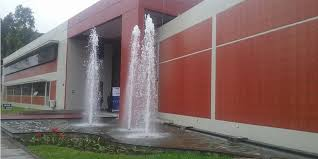
\includegraphics[scale=0.5]{ctic}}
Seguramente lo habrás aprendido en la escuela primaria: la Tierra describe una ór\-bita elíp\-tica alrededor del Sol.

Este recorrido, que se conoce como movimiento de traslación, le toma al planeta unos 365 días 
(más 5 horas, 45 minutos y 46 segundos).

El otro movimiento que te enseñaron es el de rotación: la Tierra gira en torno a su propio eje.

Este giro sobre sí misma le toma aproximadamente un día (23 horas, 56 minutos 4,1 segundos, para ser exactos). 

Sin embargo, estos no son los únicos movimientos que hace la Tierra.

\begin{sidewaysfigure}
	\centering
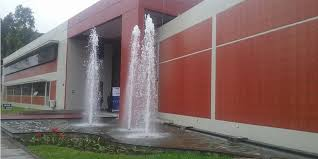
\includegraphics{ctic}
\caption*{el local de CTIC}
\end{sidewaysfigure}

El otro movimiento que te enseñaron es el de rotación: la Tierra gira en torno a su propio eje.

Este giro sobre sí misma le toma aproximadamente un día (23 horas, 56 minutos 4,1 segundos, para ser exactos). 

Sin embargo, estos no son los únicos movimientos que hace la Tierra.

El otro movimiento que te enseñaron es el de rotación: la Tierra gira en torno a su propio eje.

Este giro sobre sí misma le toma aproximadamente un día (23 horas, 56 minutos 4,1 segundos, para ser exactos). 

Sin embargo, estos no son los únicos movimientos que hace la Tierra.

El otro movimiento que te enseñaron es el de rotación: la Tierra gira en torno a su propio eje.

Este giro sobre sí misma le toma aproximadamente un día (23 horas, 56 minutos 4,1 segundos, para ser exactos). 

\begin{table}[H]
	\centering
	\caption{esto es una tabla}
	\begin{tabular}{|cc|c}
		\hline
		a & b & v \\
		d & e & f \\
		g & h & i \\
		\hline
	\end{tabular}
\end{table}

Sin embargo, estos no son los únicos movimientos que hace la Tierra.


El otro movimiento que te enseñaron es el de rotación: la Tierra gira en torno a su propio eje.

\begin{table}[H]
	\centering
	\caption{esto es una tabla esto es una tabla esto es una tabla esto es una tabla esto es una tabla}
	\begin{tabular}{|cc|c}
		\hline
		a & b & v \\
		d & e & f \\
		g & h & i \\
		\hline
	\end{tabular}
\end{table}

Este giro sobre sí misma le toma aproximadamente un día (23 horas, 56 minutos 4,1 segundos, para ser exactos). 

El otro movimiento que te enseñaron es el de rotación: la Tierra gira en torno a su propio eje.

Este giro sobre sí misma le toma aproximadamente un día (23 horas, 56 minutos 4,1 segundos, para ser exactos). 

El otro movimiento que te enseñaron es el de rotación: la Tierra gira en torno a su propio eje.

Este giro sobre sí misma le toma aproximadamente un día (23 horas, 56 minutos 4,1 segundos, para ser exactos). 

El otro movimiento que te enseñaron es el de rotación: la Tierra gira en torno a su propio eje.

Este giro sobre sí misma le toma aproximadamente un día (23 horas, 56 minutos 4,1 segundos, para ser exactos). 

El otro movimiento que te enseñaron es el de rotación: la Tierra gira en torno a su propio eje.

Este giro sobre sí misma le toma aproximadamente un día (23 horas, 56 minutos 4,1 segundos, para ser exactos). 

\begin{figure}
	\centering
\subfloat[local de ctic\label{f1a}]{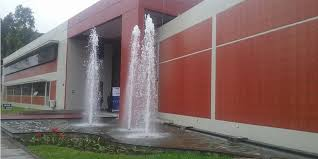
\includegraphics[scale=0.4]{ctic}}\hspace{1cm}
\subfloat[escudo de la UNI\label{f1b}]{
\includegraphics[width=3cm]{uni}}
\caption{EN LA UNIVERSIDAD EN LA UNIVERSIDAD EN LA UNIVERSIDAD EN LA UNIVERSIDAD EN LA UNIVERSIDAD EN LA UNIVERSIDAD EN LA UNIVERSIDAD}\label{f1}
\end{figure}

El otro movimiento que te enseñaron es el de rotación: la Tierra gira en torno a su propio eje.

Este giro sobre sí misma le toma aproximadamente un día (23 horas, \linebreak 56 minutos 4,1 segundos, para ser exactos). 

\pagebreak

Viendo la Figura\subref{f1a} (ctic) y la Figura \ref{f1}\subref{f1b} (escudo)

Sin embargo, estos no son los únicos movimientos que hace la Tierra.
\begin{SCfigure}[2][h]
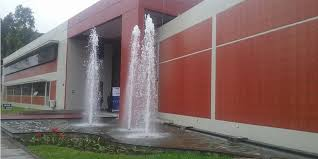
\includegraphics[scale=0.4]{ctic}
\caption{Tierra gira en torno a su propio eje gira en torno a su propio eje}
\end{SCfigure}


\end{document} \ref{f1}